\chapter{Tree}
\section{Thinking in General Trees}
{\color{blue}{Tree}} data structures usually have specific application scenarios. Unlike {\color{blue}{arrays}}, {\color{blue}{lists}}, and {\color{blue}{graphs}}, which can be seen everywhere in daily life, trees are {\color{blue}{more abstract}}. You need to get familiar with those scenarios and the corresponding solutions.

\subsection{Trees and Recursion}
{\color{ForestGreen}{Recursive algorithms are usually a natural fit for tree-based problems!}}\\
{[Reason]} Trees are {\color{blue}{hierarchical data structures}} with a {\color{blue}{parent-child relationship}}. Each {\color{blue}{subtree}} can be viewed as a {\color{blue}{tree}} itself. This mirrors the concept of {\color{blue}{recursion}} where a problem is solved by solving smaller instances of the same problem. In addition, in many problems, {\color{blue}{\ul{children of leaf nodes} or \ul{leaf nodes} are natural \ul{base cases}}}, which makes recursive algorithms easier to design.\\

Practical Tips: 
\begin{itemize}
	\item {\color{blue}{If a tree-based problem can be tackled by iteratively addressing smaller sub-problems from the root down to the leaf nodes, recursive algorithm is often a good choice.}}
	\item {\color{blue}{It's often more practical to use the \ul{children of leaf nodes} as {\color{blue}{\ul{base cases}}} instead of the leaf nodes themselves, as it's much easier to identify if a node is a child of a leaf node.}}
\end{itemize}

\subsection{Tree v.s. Graph}
A tree is a {\color{blue}{connected acyclic undirected graph}}, so in some scenarios we can consider trees in the same way as graphs. \\

For example:
\begin{itemize}
	\item {\color{blue}{Level-order traversal in trees}} is {\color{blue}{BFS in graphs}}, where the traversal begins from the root node.
	\item {\color{blue}{Pre-order traversal in trees}} is analogous to {\color{blue}{DFS in graphs}}, starting from the root and exploring the left subtree first, followed by the right subtree.
\end{itemize}

\section{Thinking in Binary Trees}
A {\color{blue}{binary tree}} is a type of tree where each node can have \ul{maximum of two children}.\\

\hdashrule[0.5ex]{\linewidth}{0.5pt}{1mm 3pt}
Unless specified, {\color{blue}{nodes}} of {\color{blue}{binary trees}} are defined as follows:
\begin{lstlisting}
struct TreeNode {
	TreeNode() : val(0), left(nullptr), right(nullptr) {}
	TreeNode(int x) : val(x), left(nullptr), right(nullptr) {}
	TreeNode(int x, TreeNode* left, TreeNode* right) : val(x), left(left), right(right) {}
	
	int val;
	TreeNode *left;
	TreeNode *right;
};
\end{lstlisting}
\hdashrule[0.5ex]{\linewidth}{0.5pt}{1mm 3pt}

\section{Thinking in Complete Binary Tree}

\section{Thinking in Balanced Binary Tree}

\section{Thinking in Binary Search Trees (BST)}
A {\color{blue}{binary search tree (BST)}} is a {\color{blue}{binary tree}} where each node has a value greater than all values in its {\color{blue}{left subtree}} and less than or equal to all values in its {\color{blue}{right subtree}}. \\

{\color{blue}{In-order traversal}} of a BST visits the nodes in a {\color{blue}{non-decreasing order}} of their values.


\section{LC 0104 - Maximum Depth of Binary Tree}
Given the root of a \ul{binary tree}, return its \ul{maximum depth}.

\subsection*{Solution - Recursion}
In this solution, we use {\color{blue}{children of leaf nodes}} as the {\color{blue}{base cases}}.
\begin{lstlisting}
int maxDepth(TreeNode* root) {
	// base case: child of leaf node
	if (!root) { return 0; }
	return std::max(maxDepth(root->left), maxDepth(root->right)) + 1;
}
\end{lstlisting}

\subsection*{*Solution - Recursion}
In this solution, we use {\color{blue}{children of leaf nodes}} and {\color{blue}{leaf nodes}} as the {\color{blue}{base cases}}.
\begin{lstlisting}
int maxDepth(TreeNode* root) {
	// base case: child of leaf node
	if (!root) { return 0; }
	// base case: leaf node
	if (!root->left && !root->right) { return 1; }
	return std::max(maxDepth(root->left), maxDepth(root->right)) + 1;
}
\end{lstlisting}

\section{LC 0111 - Minimum Depth of Binary Tree}
Given a \ul{binary tree}, find its \ul{minimum depth}.

\subsection*{Solution - Recursion}
\begin{lstlisting}
int minDepth(TreeNode* root) {
  if (!root) { return 0; }
  if (!root->left && !root->right) { return 1; }
  if (root->left && root->right) {
    return 1 + std::min(minDepth(root->left), minDepth(root->right));
  }
  if (!root->left) { return 1 + minDepth(root->right); }
  if (!root->right) { return 1 + minDepth(root->left); }
  return -1;
}
\end{lstlisting}

\subsection*{Solution 2 - Level-order Traversal}
\begin{lstlisting}
int minDepth(TreeNode* root) {
  if (!root) { return 0; }
  std::queue<std::pair<TreeNode*, int>> q;
  q.push({root, 1});
  while (!q.empty()) {
    auto [node, depth] = q.front();
    q.pop();
    if (!node->left && !node->right) { return depth; }
    if (node->left) { q.push({node->left, depth + 1}); }
    if (node->right) { q.push({node->right, depth + 1}); }
  }
  return -1;
}
\end{lstlisting}

\section{LC 0100 - Same Tree}
Given the roots of two \ul{binary trees} {\colorbox{CodeBackground}{\lstinline|p|}} and {\colorbox{CodeBackground}{\lstinline|q|}}, write a function to check if they are the same or not.\\

Two binary trees are considered the same if they are structurally identical, and the nodes have the same value.

\subsection*{Solution - Recursion}
\begin{lstlisting}
bool isSameTree(TreeNode* p, TreeNode* q) {
  // base case 1: both nodes are children of leaf nodes
  if (!p && !q) { return true; }
  // base case 2: one node is child of leaf node and the other is not
  if (!p || !q) { return false; }
  return (p->val == q->val) && isSameTree(p->left, q->left)
         && isSameTree(p->right, q->right);
}
\end{lstlisting}

\section{LC 0101 - Symmetric Tree}
Given the {\colorbox{CodeBackground}{\lstinline|root|}} of a \ul{binary tree}, check whether it is a mirror of itself (i.e., symmetric around its center).\\

A symmetric tree:
\begin{figure}[H]
	\centering
	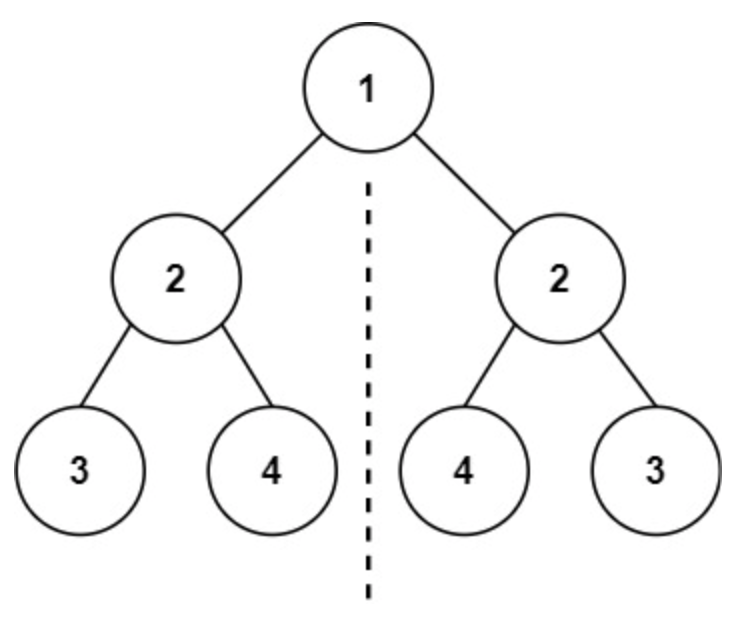
\includegraphics[width=0.25\linewidth]{images/lc0101_example}
	\label{fig:lc0101example}
\end{figure}

\subsection*{Solution - Recursion}
\begin{lstlisting}
bool isSymmetric(TreeNode* root) {
	if (!root) { return true; }
	return isSymmetricRecursive(root->left, root->right);
}

bool isSymmetricRecursive(TreeNode* t1, TreeNode* t2) {
  // base case 1: both nodes are children of leaf nodes
  if (!t1 && !t2) { return true; }
  // base case 2: one node is child of leaf node and the other is not
  if (!t1 || !t2) { return false; }
  return t1->val == t2->val && isSymmetricRecursive(t1->left, t2->right)
         && isSymmetricRecursive(t1->right, t2->left);
}
\end{lstlisting}

\section{LC 0226 - Invert Binary Tree}
Given the {\colorbox{CodeBackground}{\lstinline|root|}} of a \ul{binary tree}, invert the tree, and return its root.\\

For example:
\begin{figure}[H]
	\centering
	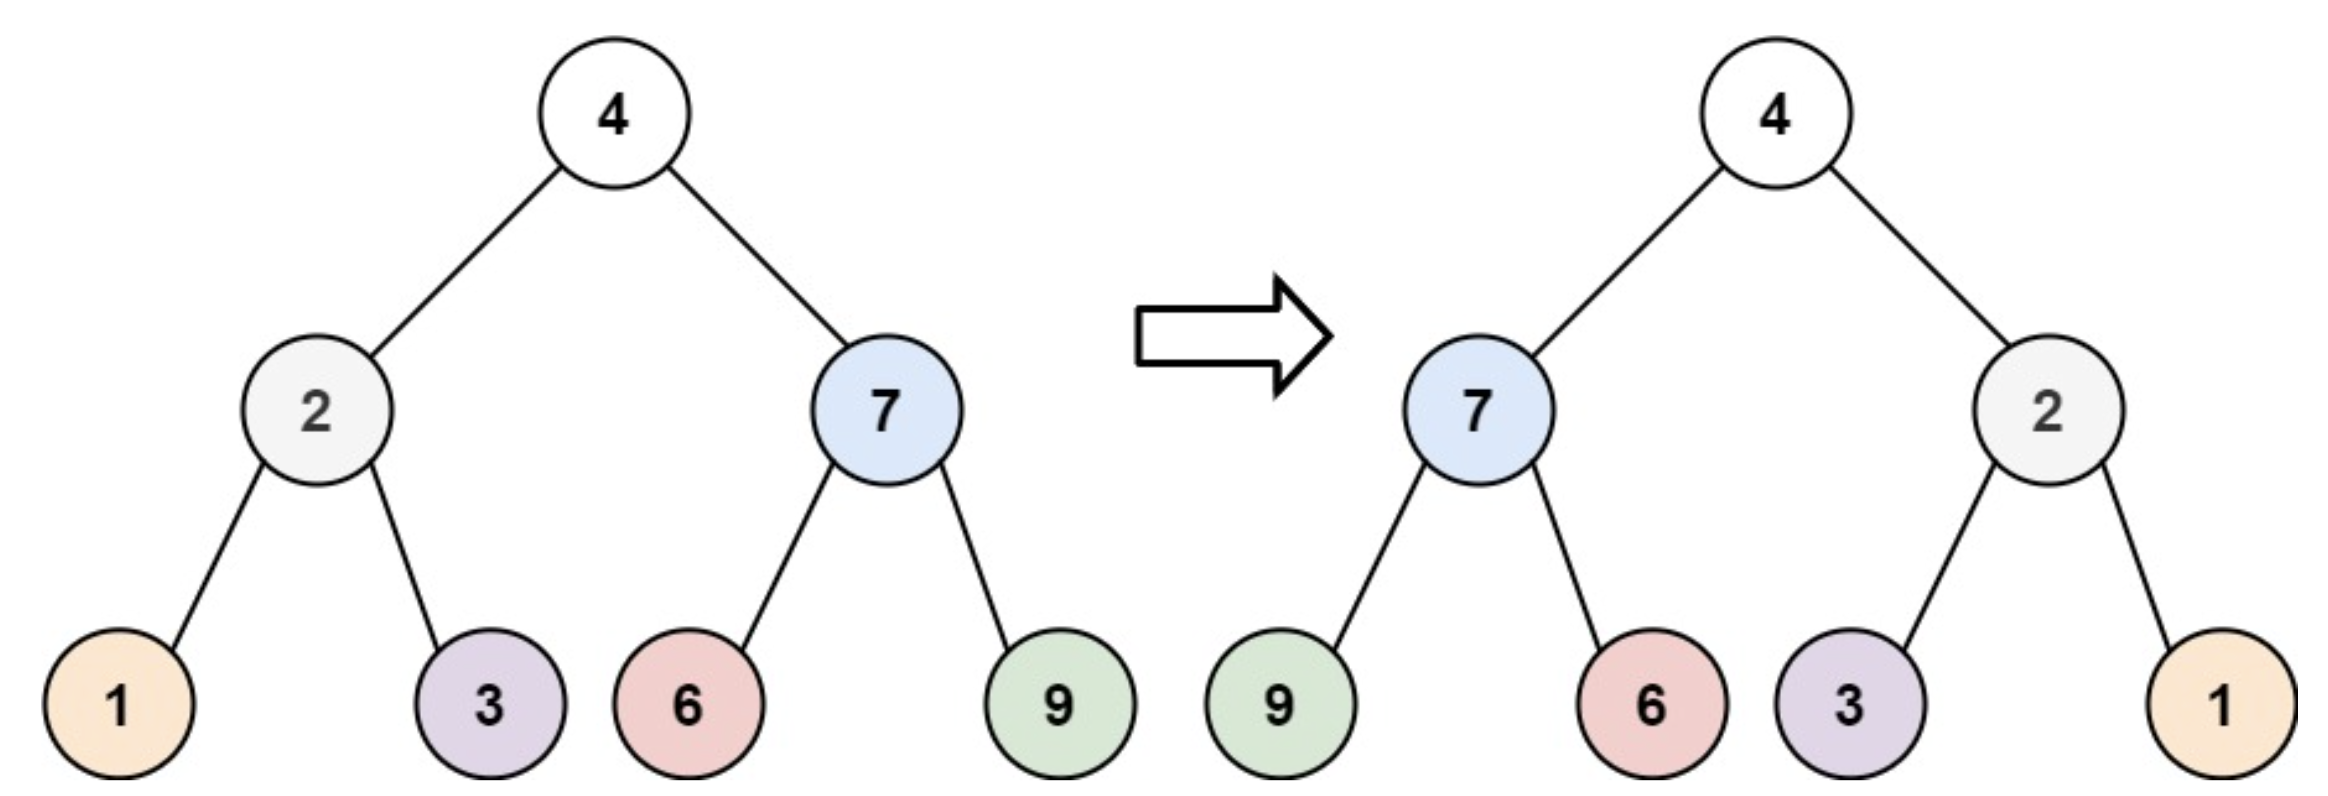
\includegraphics[width=0.7\linewidth]{images/lc0226_example}
	\label{fig:lc0226example}
\end{figure}

\subsection*{Solution - Recursion}
\begin{lstlisting}
	TreeNode* invertTree(TreeNode* root) {
		// base case: child of leaf node
		if (!root) { return root; }
		std::swap(root->left, root->right);
		invertTree(root->left);
		invertTree(root->right);
		return root;
	}
\end{lstlisting}

\section{LC 0236 - Lowest Common Ancestor of a Binary Tree}\label{lc0236}
Given a \ul{binary tree}, find the \ul{lowest common ancestor (LCA)} of two given nodes in the tree. Note that both {\colorbox{CodeBackground}{\lstinline|p|}} and {\colorbox{CodeBackground}{\lstinline|q|}} are in the tree and {\colorbox{CodeBackground}{\lstinline|p != q|}}.\\

Definition of LCA: The \ul{lowest common ancestor (LCA)} is defined between two nodes {\colorbox{CodeBackground}{\lstinline|p|}} and {\colorbox{CodeBackground}{\lstinline|q|}} as the lowest node in the tree that has both {\colorbox{CodeBackground}{\lstinline|p|}} and {\colorbox{CodeBackground}{\lstinline|q|}} as {\color{blue}{descendants}} (where we allow a node to be a {\color{blue}{descendant}} of itself). \\

Examples:
\begin{figure}[H]
	\centering
	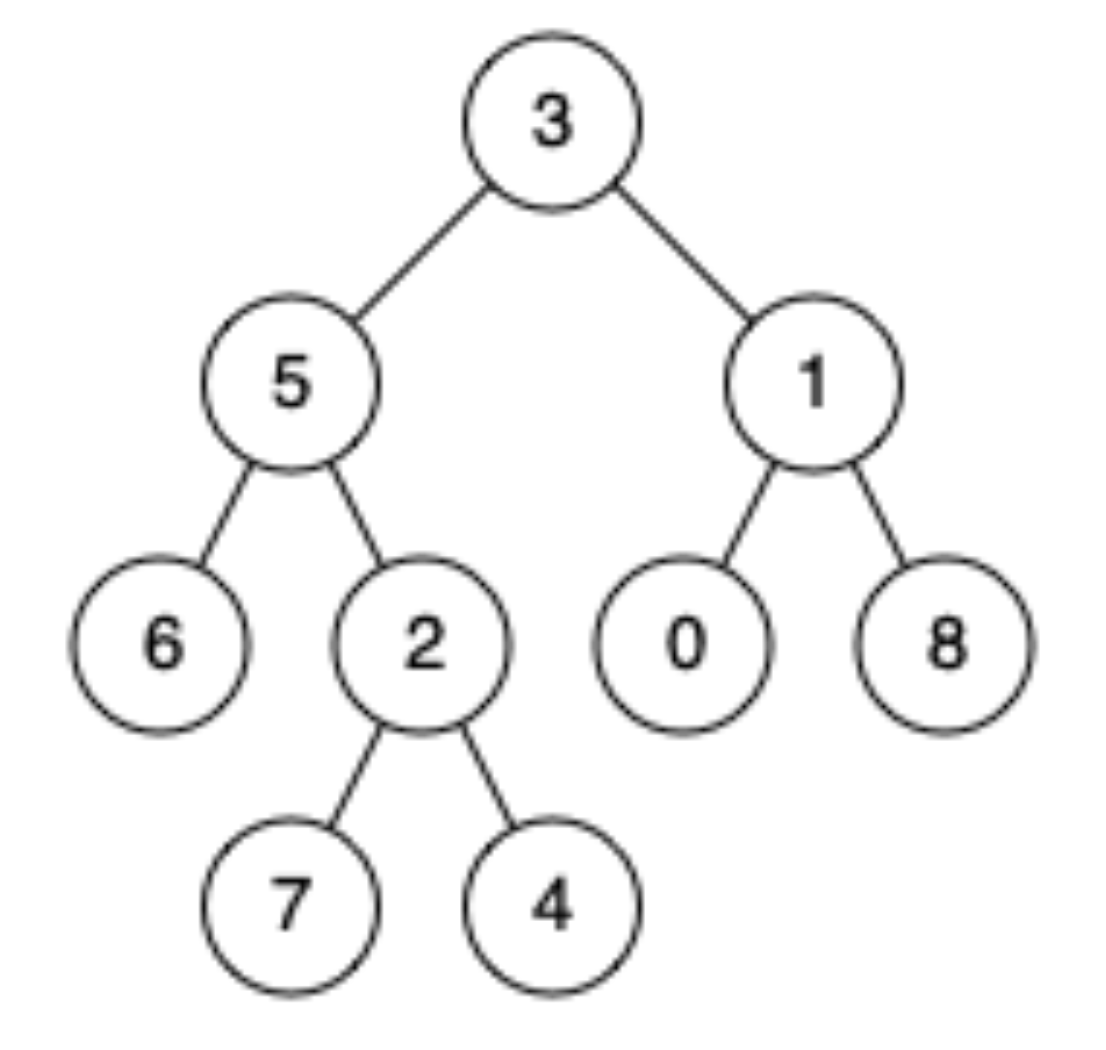
\includegraphics[width=0.3\linewidth]{images/lc0236_example_1}
	\label{fig:lc0236example1}
\end{figure}
\begin{itemize}
	\item {\colorbox{CodeBackground}{\lstinline|p = 5, q = 1 --> 3|}}
	\item {\colorbox{CodeBackground}{\lstinline|p = 5, q = 4 --> 5|}}
\end{itemize}

\subsection*{Solution - Add Parent Information}
\begin{lstlisting}
void CreateNode2Parent(TreeNode* root,
                       std::unordered_map<TreeNode*, TreeNode*>& node2parent) {
  if (!root) { return; }
  if (root->left) { node2parent[root->left] = root; }
  if (root->right) { node2parent[root->right] = root; }
  CreateNode2Parent(root->right, node2parent);
  CreateNode2Parent(root->left, node2parent);
}

TreeNode* lowestCommonAncestor(TreeNode* root, TreeNode* p, TreeNode* q) {
  if (!root) { return nullptr; }
  std::unordered_map<TreeNode*, TreeNode*> node2parent;
  node2parent[root] = nullptr;
  CreateNode2Parent(root, node2parent);
  std::vector<TreeNode*> path_p;
  while (p) {
    path_p.push_back(p);
    p = node2parent[p];
  }
  std::reverse(path_p.begin(), path_p.end());
  std::vector<TreeNode*> path_q;
  while (q) {
    path_q.push_back(q);
    q = node2parent[q];
  }
  std::reverse(path_q.begin(), path_q.end());
  TreeNode* lca = nullptr;
  int i = 0;
  while (i < std::min(path_p.size(), path_q.size()) && path_p[i] == path_q[i]) {
    lca = path_p[i];
    ++i;
  }
  return lca;
}
\end{lstlisting}

\subsection*{Solution - Recursion}
\begin{lstlisting}
// 1. both p and q are in the tree --> LCA
// 2. only one of p and q is in the tree --> that one
// 3. neither p nor q is in the tree --> nullptr
TreeNode* lowestCommonAncestor(TreeNode* root, TreeNode* p, TreeNode* q) {
	if (!root) { return nullptr; }
	if (root == p || root == q) { return root; }
	// search for LCA in left and right subtrees
	TreeNode* left = lowestCommonAncestor(root->left, p, q);
	TreeNode* right = lowestCommonAncestor(root->right, p, q);
	// if p and q are in different subtrees, return root
	if (left && right) { return root; }
	// o.w., return subtree that contains p or q
	return left ? left : right;
}
\end{lstlisting}

\subsection*{Related}
\begin{itemize}
	\item \hyperref[lc0236]{LC 0236 - Lowest Common Ancestor of a Binary Tree}
	\item \hyperref[lc0235]{LC 0235 - Lowest Common Ancestor of a BST}
\end{itemize}

\section{LC 0144 - Binary Tree Pre-order Traversal}
Given the {\colorbox{CodeBackground}{\lstinline|root|}} of a \ul{binary tree}, return the {\color{blue}{pre-order traversal}} of its nodes' values.

\subsection*{Solution - Recursion}
\begin{lstlisting}
std::vector<int> preorderTraversal(TreeNode* root) {
	static std::vector<int> res = {};
	if (!root) { return res; }
	res.push_back(root->val);
	preorderTraversal(root->left);
	preorderTraversal(root->right);
	return res;
}
\end{lstlisting}

\subsection*{Solution - Iterative}
\begin{lstlisting}
std::vector<int> preorderTraversal(TreeNode* root) {
  std::vector<int> res = {};
  if (!root) { return res; }
  std::stack<TreeNode*> stk;
  stk.push(root);
  while (!stk.empty()) {
    TreeNode* top = stk.top();
    stk.pop();
    res.push_back(top->val);
    if (top->right) { stk.push(top->right); }
    if (top->left) { stk.push(top->left); }
  }
  return res;
}
\end{lstlisting}

\section{LC 0094 - Binary Tree In-order Traversal}
Given the {\colorbox{CodeBackground}{\lstinline|root|}} of a \ul{binary tree}, return the {\color{blue}{in-order traversal}} of its nodes' values.

\subsection*{Solution - Recursion}
\begin{lstlisting}
std::vector<int> inorderTraversal(TreeNode* root) {
	static std::vector<int> res = {};
	if (!root) { return res; }
	inorderTraversal(root->left);
	res.push_back(root->val);
	inorderTraversal(root->right);
	return res;
}
\end{lstlisting}

\subsection*{Solution - Iterative}
\begin{lstlisting}
std::vector<int> inorderTraversal(TreeNode* root) {
	std::vector<int> res = {};
	if (!root) { return res; }
	std::stack<TreeNode*> stk;
	TreeNode* curr = root;
	while (curr || !stk.empty()) {
		while (curr) {
			stk.push(curr);
			curr = curr->left;
		}
		TreeNode* top = stk.top();
		stk.pop();
		res.push_back(top->val);
		curr = top->right;
	}
	return res;
}
\end{lstlisting}

\section{LC 0145 - Binary Tree Post-order Traversal}
Given the {\colorbox{CodeBackground}{\lstinline|root|}} of a \ul{binary tree}, return the {\color{blue}{post-order traversal}} of its nodes' values.

\subsection*{Solution - Recursion}
\begin{lstlisting}
std::vector<int> postorderTraversal(TreeNode* root) {
	static std::vector<int> res = {};
	if (!root) { return res; }
	postorderTraversal(root->left);
	postorderTraversal(root->right);
	res.push_back(root->val);
	return res;
}
\end{lstlisting}

\subsection*{Solution - Iterative}
\begin{lstlisting}
std::vector<int> postorderTraversal(TreeNode* root) {
	std::vector<int> res = {};
	if (!root) { return res; }
	std::stack<TreeNode*> stk;
	TreeNode* curr = root;
	TreeNode* last_visit = nullptr;
	while (curr || !stk.empty()) {
		while (curr) {
			stk.push(curr);
			curr = curr->left;
		}
		TreeNode* top = stk.top();
		if (top->right && top->right != last_visit) {
			// right node exists && right node is not visited
			curr = top->right;
		} else {
			// right node does not exist || right node is visited
			// handle the node, e.g., print it
			res.push_back(top->val);
			last_visit = top;
			stk.pop();
		}
	}
	return res;
}
\end{lstlisting}

\section{LC 0105 - Construct Binary Tree from Pre-order and In-order Traversal}
Given two integer arrays {\colorbox{CodeBackground}{\lstinline|preorder|}} and {\colorbox{CodeBackground}{\lstinline|inorder|}} where {\colorbox{CodeBackground}{\lstinline|preorder|}} is the \ul{pre-order traversal} of a \ul{binary tree} and {\colorbox{CodeBackground}{\lstinline|inorder|}} is the \ul{in-order traversal} of the same tree, construct and return the binary tree. It should be noted that {\colorbox{CodeBackground}{\lstinline|preorder|}} and {\colorbox{CodeBackground}{\lstinline|inorder|}} consist of unique values. \\

Example:
\begin{figure}[H]
	\centering
	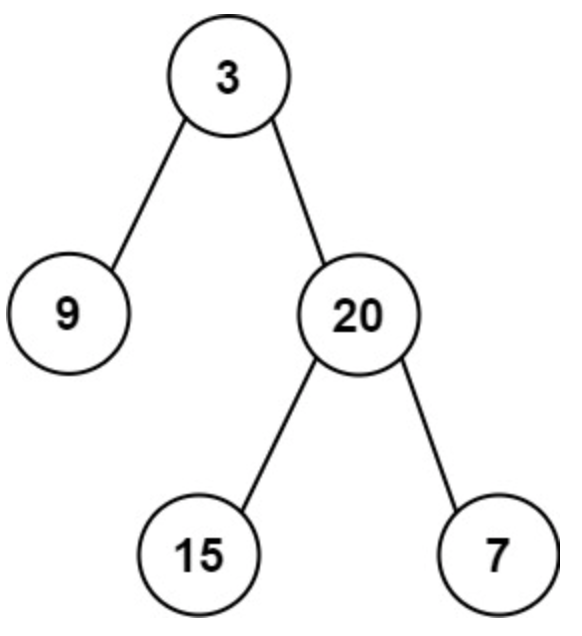
\includegraphics[width=0.23\linewidth]{images/lc0105_example}
	\label{fig:lc0105example}
\end{figure}
{\colorbox{CodeBackground}{\lstinline|preorder = [3,9,20,15,7], inorder = [9,3,15,20,7] --> [3,9,20,nullptr,nullptr,15,7]|}}

\subsection*{Solution}
The steps are as follows:
\begin{enumerate}
	\item Use the {\color{blue}{first element}} of the {\colorbox{CodeBackground}{\lstinline|preorder|}} array to identify the {\color{blue}{root}}.
	\item Find this root in the {\colorbox{CodeBackground}{\lstinline|inorder|}} array. Elements to the left are part of the {\color{blue}{left subtree}}, and elements to the right are part of the {\color{blue}{right subtree}}.
	\item Recursively apply this logic to build the left and right subtrees.
\end{enumerate}
\begin{lstlisting}
TreeNode* buildTree(std::vector<int>& preorder, std::vector<int>& inorder) {
	std::unordered_map<int, int> in_val2idx;
	for (int i = 0; i < inorder.size(); i++) { in_val2idx[inorder[i]] = i; }
	return buildTreeRecursive(preorder, 0, preorder.size() - 1, inorder, 0, inorder.size() - 1,
	in_val2idx);
}

TreeNode* buildTreeRecursive(std::vector<int>& preorder, int pre_start, int pre_end,
std::vector<int>& inorder, int in_start, int in_end,
std::unordered_map<int, int>& in_val2idx) {
	// base case
	if (pre_start > pre_end || in_start > in_end) { return nullptr; }
	TreeNode* root = new TreeNode(preorder[pre_start]);
	int in_root = in_val2idx[root->val];
	int num_left = in_root - in_start;
	root->left = buildTreeRecursive(preorder, pre_start + 1, pre_start + num_left, inorder, 
	in_start, in_root - 1, in_val2idx);
	root->right = buildTreeRecursive(preorder, pre_start + num_left + 1, pre_end, 
	inorder, in_root + 1, in_end, in_val2idx);
	
	return root;
}
\end{lstlisting}

\section{LC 0106 - Construct Binary Tree from In-order and Post-order Traversal}
Given two integer arrays {\colorbox{CodeBackground}{\lstinline|inorder|}} and {\colorbox{CodeBackground}{\lstinline|postorder|}} where {\colorbox{CodeBackground}{\lstinline|inorder|}} is the \ul{in-order traversal} of a \ul{binary tree} and {\colorbox{CodeBackground}{\lstinline|postorder|}} is the \ul{post-order traversal} of the same tree, construct and return the binary tree. It should be noted that {\colorbox{CodeBackground}{\lstinline|inorder|}} and {\colorbox{CodeBackground}{\lstinline|postorder|}} consist of unique values.  \\

Example:
\begin{figure}[H]
	\centering
	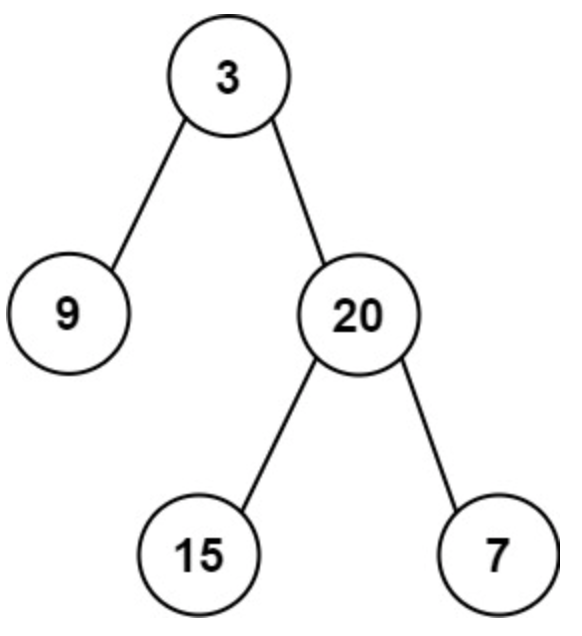
\includegraphics[width=0.23\linewidth]{images/lc0105_example}
	\label{fig:lc0106example}
\end{figure}
{\colorbox{CodeBackground}{\lstinline|inorder = [9,3,15,20,7], postorder = [9,15,7,20,3] --> [3,9,20,null,null,15,7]|}}

\subsection*{Solution}
The steps are as follows:
\begin{enumerate}
	\item Use the {\color{blue}{last element}} of the {\colorbox{CodeBackground}{\lstinline|postorder|}} array as the {\color{blue}{root}}.
	\item Find this root in the {\colorbox{CodeBackground}{\lstinline|inorder|}} array. Elements to the left are part of the {\color{blue}{left subtree}}, and elements to the right are part of the {\color{blue}{right subtree}}.
	\item Recursively apply this logic to build the left and right subtrees.
\end{enumerate}

\begin{lstlisting}
TreeNode* buildTree(std::vector<int>& inorder, std::vector<int>& postorder) {
	std::unordered_map<int, int> in_val2idx;
	for (int i = 0; i < inorder.size(); i++) { in_val2idx[inorder[i]] = i; }
	return buildTreeRecursive(inorder, 0, inorder.size() - 1, postorder, 0,
	postorder.size() - 1, in_val2idx);
}

TreeNode* buildTreeRecursive(std::vector<int>& inorder, int in_start, int in_end,
std::vector<int>& postorder, int post_start, int post_end,
std::unordered_map<int, int>& in_val2idx) {
	// base case
	if (in_start > in_end || post_start > post_end) { return nullptr; }
	TreeNode* root = new TreeNode(postorder[post_end]);
	int in_root = in_val2idx[root->val];
	int num_left = in_root - in_start;
	root->left = buildTreeRecursive(inorder, in_start, in_root - 1, postorder, post_start,
	post_start + num_left - 1, in_val2idx);
	root->right = buildTreeRecursive(inorder, in_root + 1, in_end, postorder, 
	post_start + num_left, post_end - 1, in_val2idx);
	return root;
}
\end{lstlisting}

\section{LC 0114 - Flatten Binary Tree to Linked List}
Given the {\colorbox{CodeBackground}{\lstinline|root|}} of a \ul{binary tree}, flatten the tree into a \ul{linked list}:
\begin{itemize}
	\item The linked list should use the same {\colorbox{CodeBackground}{\lstinline|TreeNode|}} class where the {\colorbox{CodeBackground}{\lstinline|right|}} child pointer points to the next node in the list and the left child pointer is always {\colorbox{CodeBackground}{\lstinline|nullptr|}}.
	\item The linked list should be in the same order as a \ul{pre-order traversal} of the binary tree.
\end{itemize}

Example:

\begin{figure}[H]
	\centering
	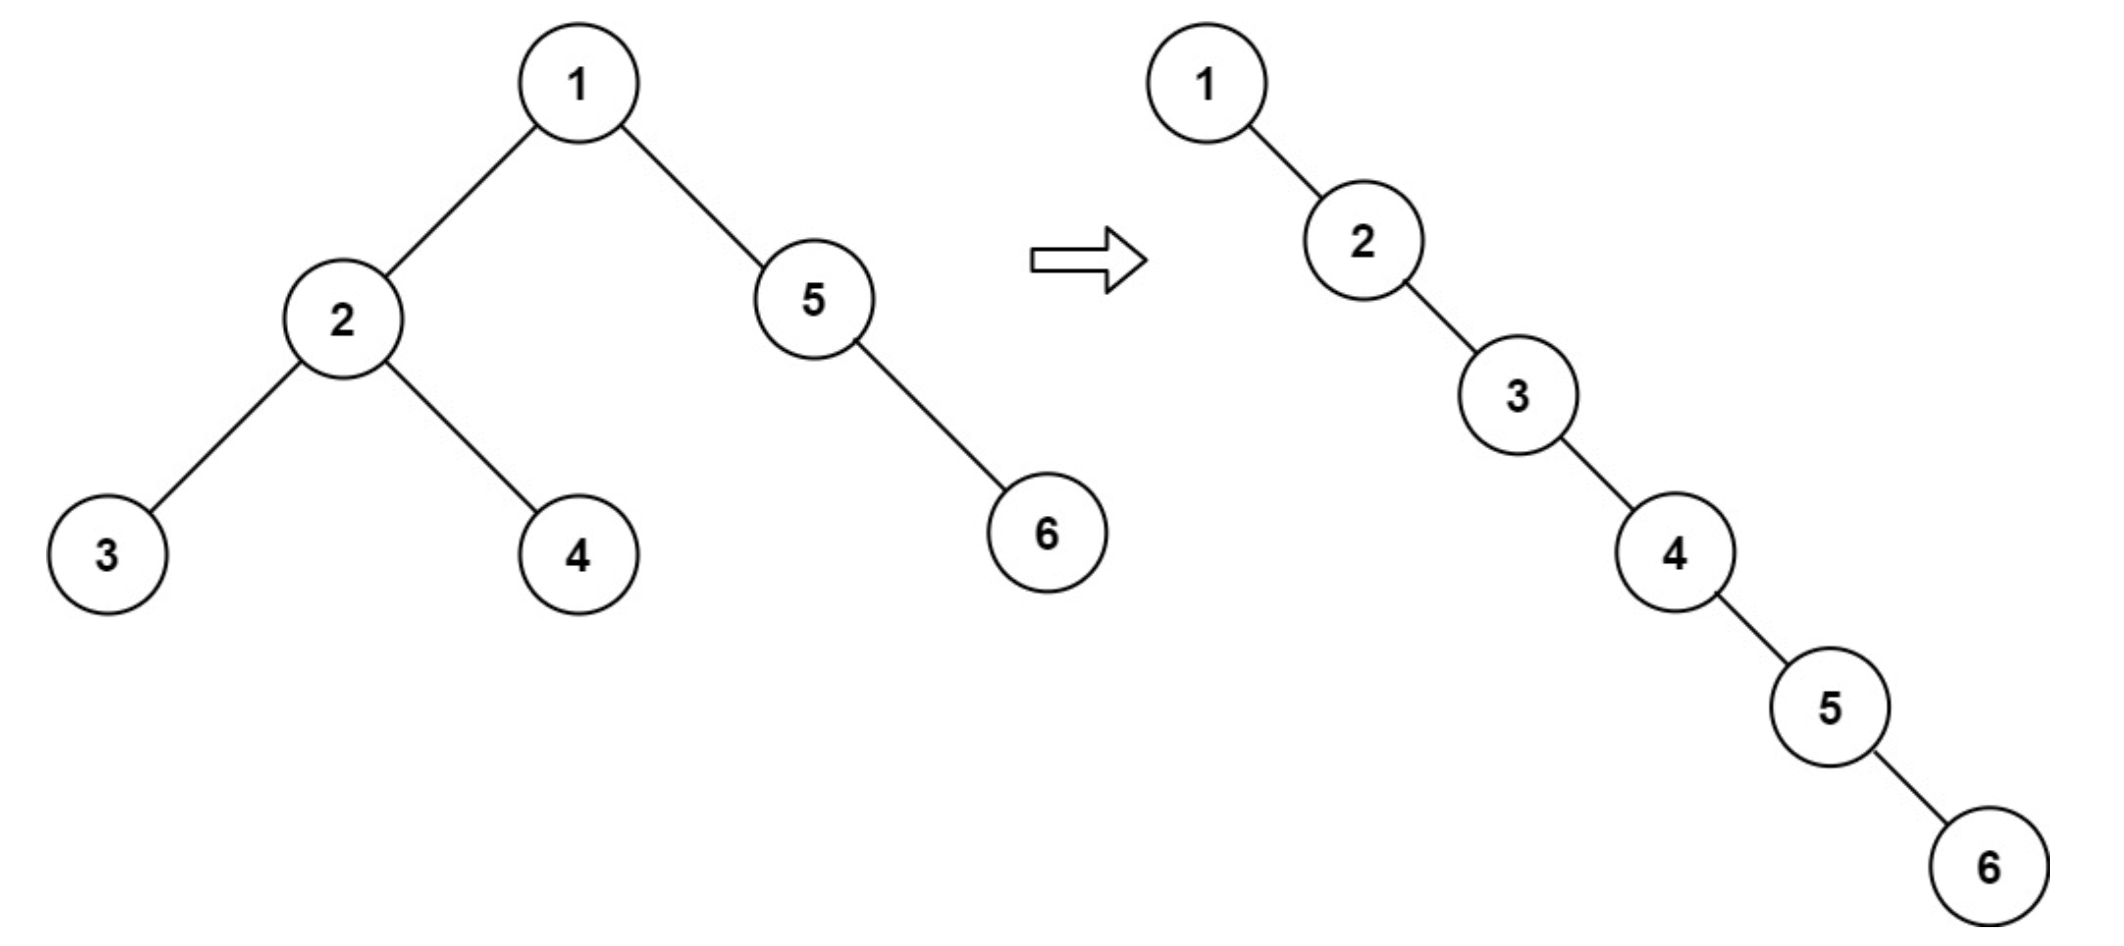
\includegraphics[width=0.8\linewidth]{images/lc0114_example}
	\label{fig:lc0114example}
\end{figure}

\subsection*{Solution - Recursion}
\begin{lstlisting}
void flatten(TreeNode* root) {
	// base case
	if (!root) { return; }
	flatten(root->left);
	flatten(root->right);
	// temporarily store the right child as it will be overwritten.
	TreeNode* temp_right = root->right;
	if (root->left) {
		// attach the left subtree to the right of the root
		root->right = root->left;
		root->left = nullptr;
		// attach the original right subtree to the tail of the new right subtree
		TreeNode* curr = root->right;
		while (curr->right) { curr = curr->right; }
		curr->right = temp_right;
	}
}
\end{lstlisting}

\section{LC 0102 - Binary Tree Level Order Traversal}
Given the {\colorbox{CodeBackground}{\lstinline|root|}} of a \ul{binary tree}, return the level order traversal of its nodes' values. (i.e., from left to right, level by level).\\

Example:
\begin{figure}[H]
	\centering
	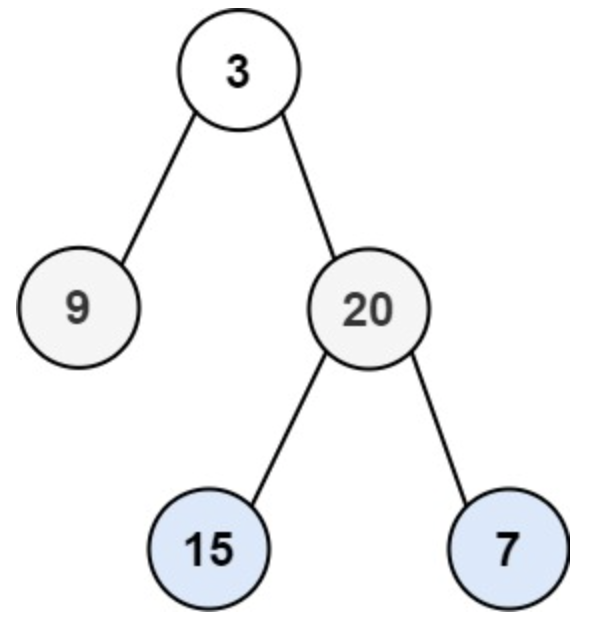
\includegraphics[width=0.25\linewidth]{images/lc0102_example}
	\label{fig:lc0102example}
\end{figure}
{\colorbox{CodeBackground}{\lstinline|--> [[3],[9,20],[15,7]]|}}

\subsection*{Solution}
\begin{lstlisting}
std::vector<std::vector<int>> levelOrder(TreeNode* root) {
	std::vector<std::vector<int>> result;
	if (!root) { return result; }
	std::queue<TreeNode*> q;
	q.push(root);
	while (!q.empty()) {
		int level_size = q.size();
		std::vector<int> curr_level;
		for (int i = 0; i < level_size; ++i) {
			TreeNode* node = q.front();
			q.pop();
			curr_level.push_back(node->val);
			if (node->left) { q.push(node->left); }
			if (node->right) { q.push(node->right); }
		}
		result.push_back(curr_level);
	}
	return result;
}
\end{lstlisting}

\section{LC 0103 - Binary Tree Zigzag Level Order Traversal}
Given the {\colorbox{CodeBackground}{\lstinline|root|}} of a \ul{binary tree}, return the \ul{zigzag level order traversal} of its nodes' values. (i.e., from left to right, then right to left for the next level and alternate between).\\

Example:
\begin{figure}[H]
	\centering
	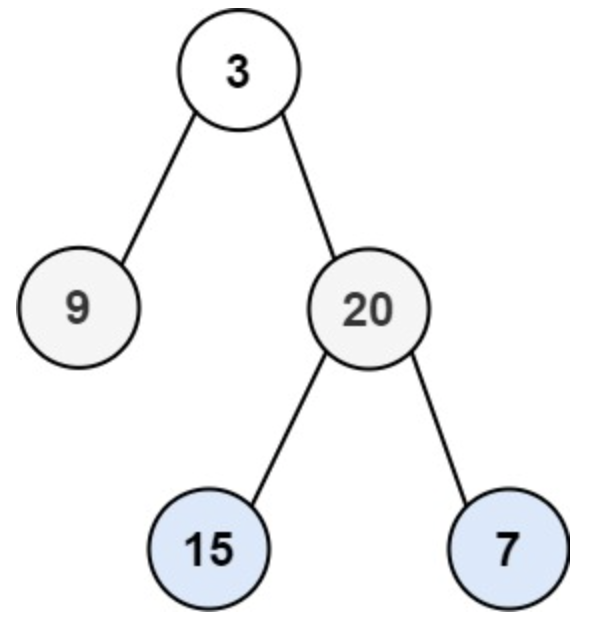
\includegraphics[width=0.25\linewidth]{images/lc0102_example}
	\label{fig:lc0102example}
\end{figure}
{\colorbox{CodeBackground}{\lstinline|--> [[3],[20,9],[15,7]]|}}

\subsection*{Solution}
\begin{lstlisting}
std::vector<std::vector<int>> zigzagLevelOrder(TreeNode* root) {
	std::vector<std::vector<int>> result;
	if (!root) { return result; }
	std::queue<TreeNode*> q;
	q.push(root);
	bool l2r = true;
	while (!q.empty()) {
		int level_size = q.size();
		std::vector<int> cur_level(level_size);
		for (int i = 0; i < level_size; ++i) {
			TreeNode* node = q.front();
			q.pop();
			int idx = (l2r) ? i : (level_size - 1 - i);
			cur_level[idx] = node->val;
			if (node->left) { q.push(node->left); }
			if (node->right) { q.push(node->right); }
		}
		l2r = !l2r;
		result.push_back(cur_level);
	}
	return result;
}
\end{lstlisting}

\section{LC 0637 - Average of Levels in Binary Tree}
Given the {\colorbox{CodeBackground}{\lstinline|root|}} of a \ul{binary tree}, return the average value of the nodes on each level in the form of an array.\\

Example:
\begin{figure}[H]
	\centering
	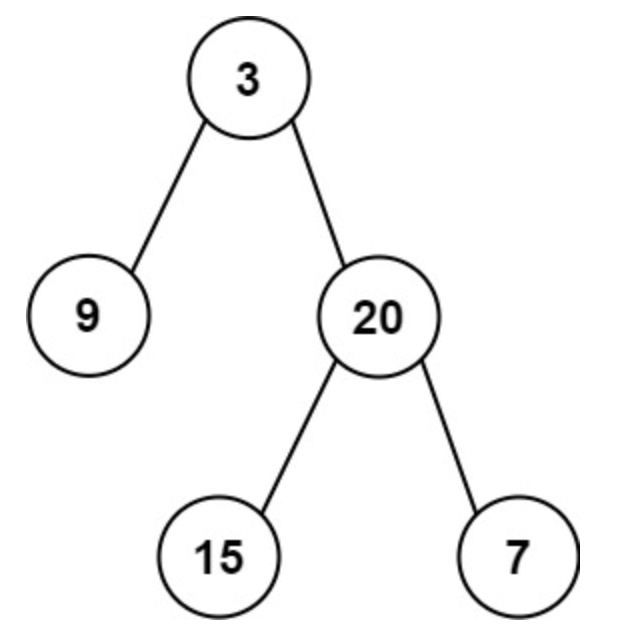
\includegraphics[width=0.25\linewidth]{images/lc0637_example}
	\label{fig:lc0637example}
\end{figure}
{\colorbox{CodeBackground}{\lstinline|--> [3.00000,14.50000,11.00000]|}}

\subsection*{Solution}
level-order traversal
\begin{lstlisting}
std::vector<double> averageOfLevels(TreeNode* root) {
	std::vector<double> avg_level;
	std::queue<TreeNode*> q;
	q.push(root);
	while (!q.empty()) {
		int level_size = q.size();
		double level_sum = 0;
		for (int i = 0; i < level_size; ++i) {
			TreeNode* curr = q.front();
			q.pop();
			level_sum += curr->val;
			if (curr->left) { q.push(curr->left); }
			if (curr->right) { q.push(curr->right); }
		}
		avg_level.push_back(level_sum / level_size);
	}
	return avg_level;
}
\end{lstlisting}

\section{LC 0199 - Binary Tree Right Side View}
Given the {\colorbox{CodeBackground}{\lstinline|root|}} of a \ul{binary tree}, imagine yourself standing on the right side of it, return the values of the nodes you can see ordered from top to bottom.\\

Example:
\begin{figure}[H]
	\centering
	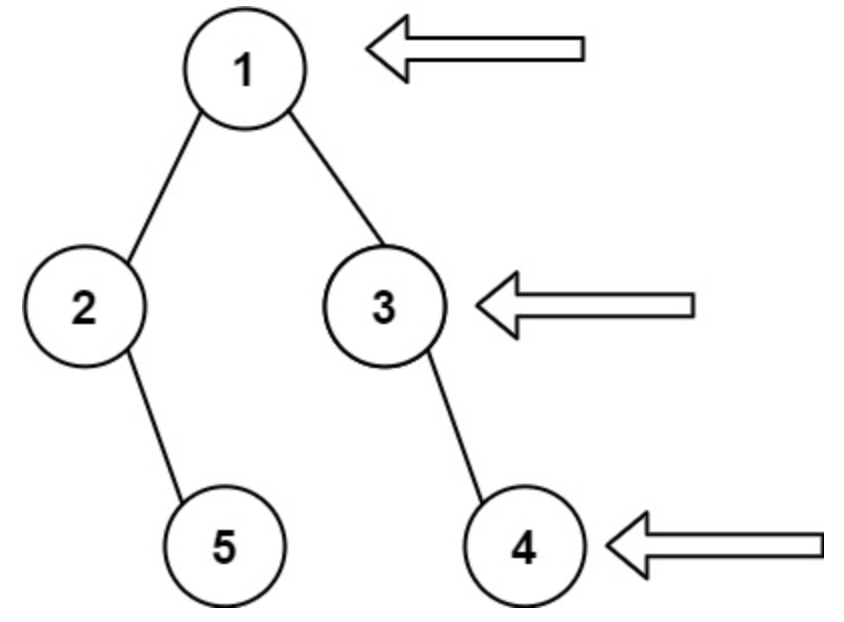
\includegraphics[width=0.33\linewidth]{images/lc0199_example}
	\label{fig:lc0199example}
\end{figure}
{\colorbox{CodeBackground}{\lstinline|--> [1,3,4]|}}

\subsection*{Solution - Iterative}
level-order traversal
\begin{lstlisting}
std::vector<int> rightSideView(TreeNode* root) {
	if (!root) { return; };
	std::vector<int> view;
	std::queue<TreeNode*> q;
	q.push(root);
	while (!q.empty()) {
		int level_size = q.size();
		for (int i = 0; i < level_size; ++i) {
			TreeNode* node = q.front();
			q.pop();
			if (i == level_size - 1) { view.push_back(node->val); }
			if (node->left) { q.push(node->left); }
			if (node->right) { q.push(node->right); }
		}
	}
	return view;
}
\end{lstlisting}

\subsection*{Solution - Recursion}
\begin{lstlisting}
std::vector<int> rightSideView(TreeNode* root) {
	std::vector<int> view;
	rightViewDFS(root, 0, view);
	return view;
}

void rightViewDFS(TreeNode* node, int level, std::vector<int>& view) {
	if (!node) { return; }
	// first time we've reached this level
	if (level == view.size()) { view.push_back(node->val); }
	// prioritize right subtree, then left subtree.
	rightViewDFS(node->right, level + 1, view);
	rightViewDFS(node->left, level + 1, view);
}
\end{lstlisting}

\section{LC 0117 - Populating Next Right Pointers in Each Node II}
Given a \ul{binary tree}:
\begin{lstlisting}
struct Node {
	int val;
	Node *left;
	Node *right;
	Node *next;
};
\end{lstlisting}
Populate each next pointer to point to its next right node. If there is no next right node, the next pointer should be set to {\colorbox{CodeBackground}{\lstinline|nullptr|}}. Initially, all next pointers are set to {\colorbox{CodeBackground}{\lstinline|nullptr|}}.\\

Example:
\begin{figure}[H]
	\centering
	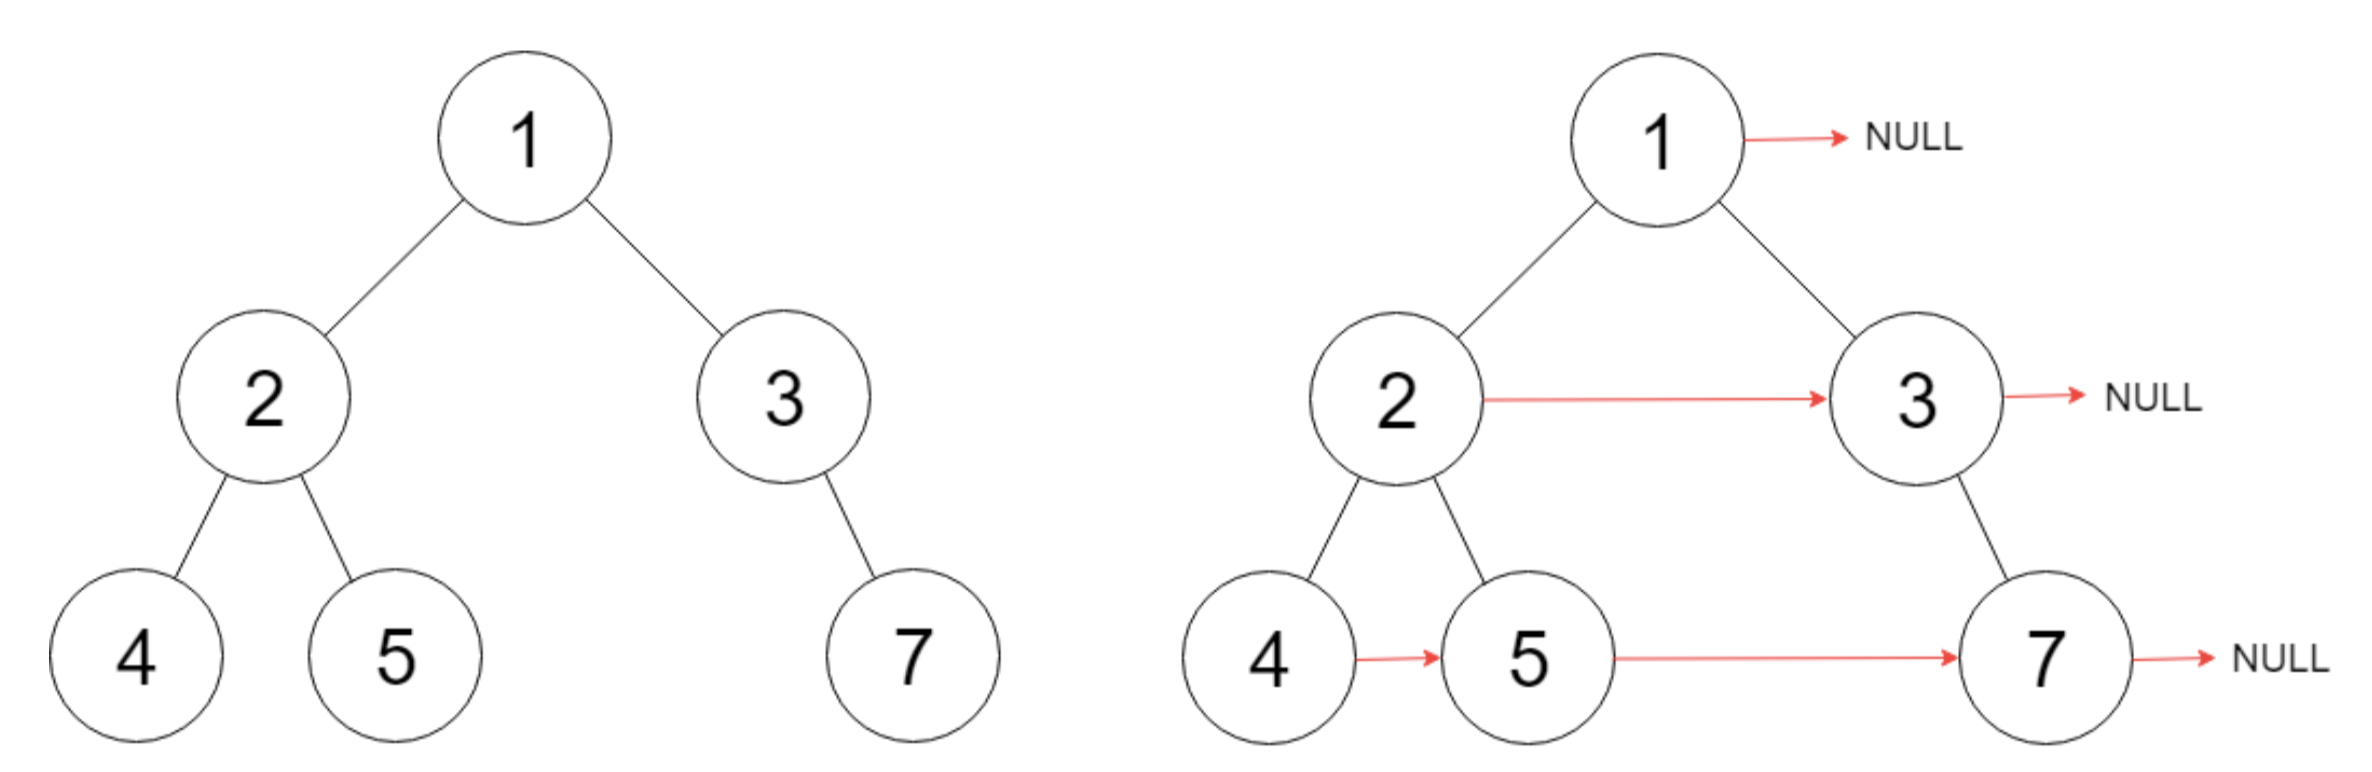
\includegraphics[width=0.65\linewidth]{images/lc0117_example}
	\label{fig:lc0117example}
\end{figure}

\subsection*{Solution}
level-order traversal
\begin{lstlisting}
Node* connect(Node* root) {
	if (!root) { return root; }
	std::queue<Node*> q;
	q.push(root);
	while (!q.empty()) {
		Node* prev = nullptr;
		int level_size = q.size();
		for (int i = 0; i < level_size; ++i) {
			Node* curr = q.front();
			q.pop();
			if (prev) { prev->next = curr; }
			prev = curr;
			if (curr->left) { q.push(curr->left); }
			if (curr->right) { q.push(curr->right); }
		}
		prev->next = nullptr;
	}
	return root;
}
\end{lstlisting}

\section{LC 0112 - Path Sum}\label{lc0112}
Given the {\colorbox{CodeBackground}{\lstinline|root|}} of a \ul{binary tree} and an integer {\colorbox{CodeBackground}{\lstinline|targetSum|}}, return {\colorbox{CodeBackground}{\lstinline|true|}} if the tree has a \ul{root-to-leaf path} such that adding up all the values along the path equals {\colorbox{CodeBackground}{\lstinline|targetSum|}}.\\

Example:
\begin{figure}[H]
	\centering
	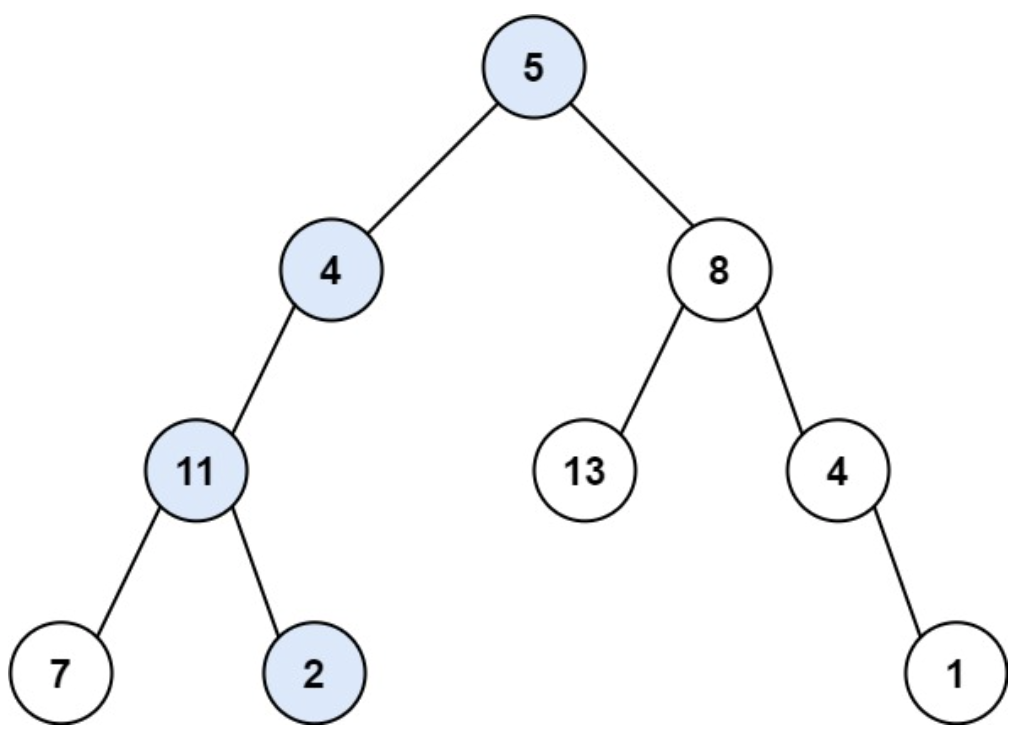
\includegraphics[width=0.5\linewidth]{images/lc0112}
	\label{fig:lc0112}
\end{figure}
{\colorbox{CodeBackground}{\lstinline|root = [5,4,8,11,null,13,4,7,2,null,null,null,1], targetSum = 22 --> true|}}

\subsection*{Solution - Recursion}
\begin{lstlisting}
bool hasPathSum(TreeNode* root, int targetSum) {
	// base case 1: child of leaf node
	if (!root) { return false; }
	// base case 2: leaf node
	if (!root->left && !root->right) { return root->val == targetSum; }
	return hasPathSum(root->left, targetSum - root->val)
	|| hasPathSum(root->right, targetSum - root->val);
}
\end{lstlisting}

\subsection*{Related}
\begin{itemize}
	\item \hyperref[lc0120]{[Binary Tree] LC 0120 - Triangle}
	\item \hyperref[lc0112]{[Binary Tree] LC 0112 - Path Sum}
	\item \hyperref[lc0124]{[Binary Tree] LC 0124 - Binary Tree Maximum Path Sum}
	\item \hyperref[lc0064]{[Matrix] LC 0064 - Minimum Path Sum}
\end{itemize}

\section{LC 0129 - Sum Root to Leaf Numbers}
You are given the {\colorbox{CodeBackground}{\lstinline|root|}} of a \ul{binary tree} containing digits from {\colorbox{CodeBackground}{\lstinline|0|}} to {\colorbox{CodeBackground}{\lstinline|9|}} only.\\

Each \ul{root-to-leaf path} in the tree represents a number.\\

For example, the \ul{root-to-leaf path} {\colorbox{CodeBackground}{\lstinline|1 --> 2 --> 3|}} represents the number {\colorbox{CodeBackground}{\lstinline|123|}}.\\

Return the total sum of all \ul{root-to-leaf numbers}.\\

Example:
\begin{figure}[H]
	\centering
	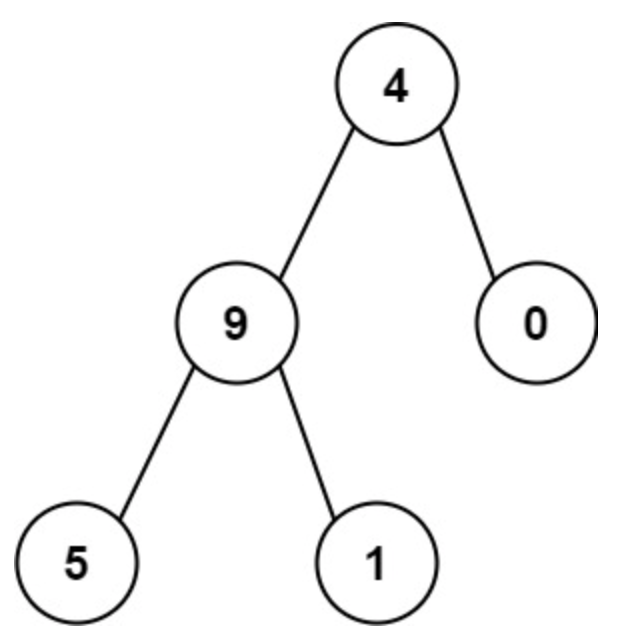
\includegraphics[width=0.23\linewidth]{images/lc0129_example}
	\label{fig:lc0129example}
\end{figure}
{\colorbox{CodeBackground}{\lstinline|root = [4,9,0,5,1] --> 1026 (495 + 491 + 40)|}}

\subsection*{Solution}
\begin{lstlisting}
int sumNumbers(TreeNode* root) { return sumNumbersRecursive(root, 0); }

int sumNumbersRecursive(TreeNode* node, int cur_sum) {
	// base case 1: child of leaf node
	if (!node) { return 0; }
	cur_sum = cur_sum * 10 + node->val;
	// base case 2: leaf node
	if (!node->left && !node->right) { return cur_sum; }
	return sumNumbersRecursive(node->left, cur_sum) 
	+ sumNumbersRecursive(node->right, cur_sum);
}
\end{lstlisting}

\section{LC 0124 - Binary Tree Maximum Path Sum}\label{lc0124}
A \ul{path} in a \ul{binary tree} is a sequence of nodes where each pair of \ul{adjacent nodes} in the sequence has an \ul{edge} connecting them. A node can only appear in the sequence at most once. Note that the path does not need to pass through the root.\\

The \ul{path sum} of a path is the sum of the node's values in the path.\\

Given the {\colorbox{CodeBackground}{\lstinline|root|}} of a binary tree, return the \ul{maximum path sum} of any non-empty path.\\

Example:
\begin{figure}[H]
	\centering
	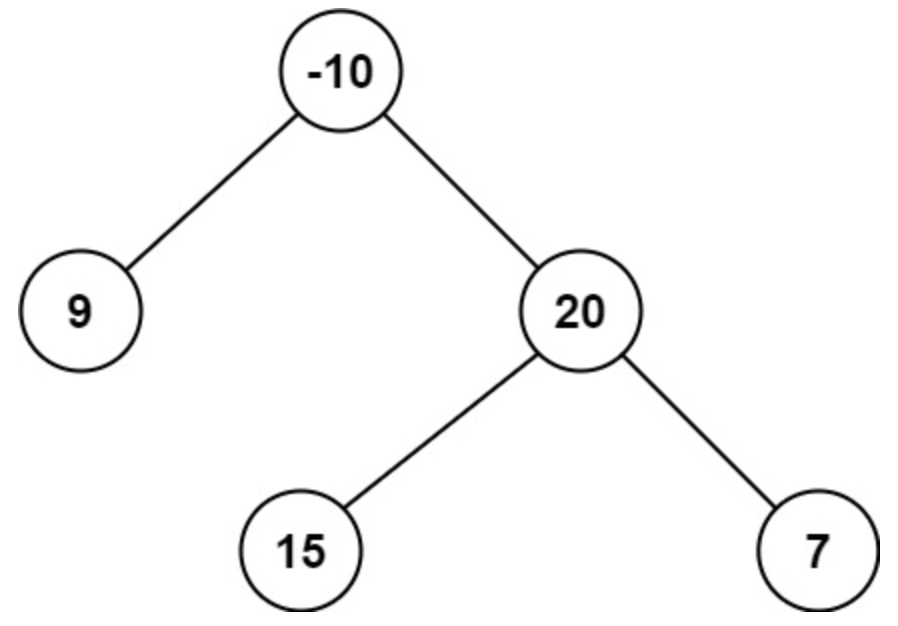
\includegraphics[width=0.35\linewidth]{images/lc0124_example}
	\label{fig:lc0124example}
\end{figure}
{\colorbox{CodeBackground}{\lstinline|root = [-10,9,20,null,null,15,7] --> 42 (15 + 20 + 7)|}}

\subsection*{Solution}
The recursive function {\colorbox{CodeBackground}{\lstinline|maxPathDown|}} does more than just calculate the maximum path sum starting from the root. More importantly, it explores all potential paths throughout the tree, evaluating each for the maximum path sum we're seeking.
\begin{lstlisting}
int maxPathSum(TreeNode* root) {
	int max_sum = std::numeric_limits<int>::min();
	maxPathDown(root, max_sum);
	return max_sum;
}

// calculate maximum path sum starting from root and update max_sum
int maxPathDown(TreeNode* root, int& max_sum) {
	// base case: child of leaf node
	if (!root) { return 0; }
	// maximum path sum starting from left and right child, set to zero if negative
	int left = std::max(0, maxPathDown(root->left, max_sum));
	int right = std::max(0, maxPathDown(root->right, max_sum));
	// update max_sum
	max_sum = std::max(max_sum, root->val + left + right);
	// return maximum path sum starting from root
	return std::max(left, right) + root->val;
}
\end{lstlisting}

\subsection*{Related}
\begin{itemize}
	\item \hyperref[lc0120]{[Binary Tree] LC 0120 - Triangle}
	\item \hyperref[lc0112]{[Binary Tree] LC 0112 - Path Sum}
	\item \hyperref[lc0124]{[Binary Tree] LC 0124 - Binary Tree Maximum Path Sum}
	\item \hyperref[lc0064]{[Matrix] LC 0064 - Minimum Path Sum}
\end{itemize}

\section{LC 0958 - Check Completeness of a Binary Tree}\label{lc0958}
Given the root of a binary tree, determine if it is a \ul{complete binary tree}.

\subsection*{Solution}
level-order traversal $+$ state {\colorbox{CodeBackground}{\lstinline|bool null_seen|}}
\begin{lstlisting}
int countNodes(TreeNode* root) {
	if (!root) { return 0; }
	int left_h = 0;
	int right_h = 0;
	TreeNode* left = root;
	TreeNode* right = root;
	while (left) {
		++left_h;
		left = left->left;
	}
	while (right) {
		++right_h;
		right = right->right;
	}
	// full binary tree
	if (left_h == right_h) { return (1 << left_h) - 1; }
	// non-full complete binary tree
	return 1 + countNodes(root->left) + countNodes(root->right);
}
\end{lstlisting}

\subsection*{Related}
\begin{itemize}
	\item \hyperref[lc0958]{LC 0958 - Check Completeness of a Binary Tree}
	\item \hyperref[lc0098]{LC 0098 - Validate BST}
\end{itemize}

\section{LC 0222 - Count Complete Tree Nodes}
Given the {\colorbox{CodeBackground}{\lstinline|root|}} of a \ul{complete binary tree}, return the number of the nodes in the tree.\\

Design an algorithm that runs in less than {\colorbox{CodeBackground}{\lstinline|O(n)|}} time complexity where {\colorbox{CodeBackground}{\lstinline|n|}} is the number of nodes of the tree.\\

Example:
\begin{figure}[H]
	\centering
	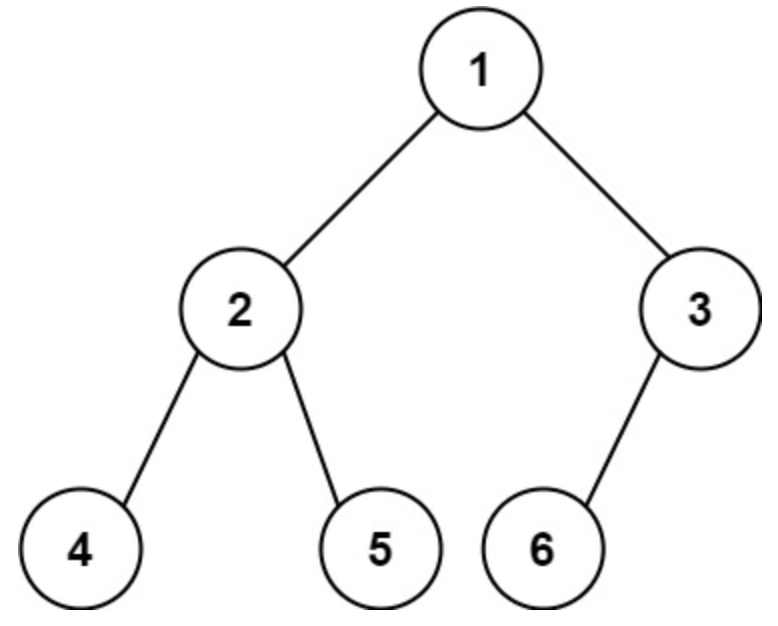
\includegraphics[width=0.32\linewidth]{images/lc0222_example}
	\label{fig:lc0222example}
\end{figure}
{\colorbox{CodeBackground}{\lstinline|--> 6|}}

\subsection*{Solution - Recursion}
\begin{lstlisting}
int countNodes(TreeNode* root) {
	if (!root) { return 0; }
	int left_h = 0;
	int right_h = 0;
	TreeNode* left = root;
	TreeNode* right = root;
	while (left) {
		++left_h;
		left = left->left;
	}
	while (right) {
		++right_h;
		right = right->right;
	}
	// base case: full binary tree
	if (left_h == right_h) { return (1 << left_h) - 1; }
	// non-full complete binary tree
	return 1 + countNodes(root->left) + countNodes(root->right);
}
\end{lstlisting}

\section{LC 0098 - Validate BST}\label{lc0098}
Given the {\colorbox{CodeBackground}{\lstinline|root|}} of a \ul{binary tree}, determine if it is a valid \ul{binary search tree (BST)}.\\

A valid BST is defined as follows:
\begin{itemize}
	\item The left subtree of a node contains only nodes with keys less than the node's key.
	\item The right subtree of a node contains only nodes with keys greater than the node's key.
	\item Both the left and right subtrees must also be binary search trees.
\end{itemize}

\subsection*{Solution 1 - In-order Traversal (Recursive)}
\begin{lstlisting}
bool isValidBST(TreeNode* root) {
	long prev_val = LONG_MIN;
	return InorderCheck(root, prev_val);
}

bool InorderCheck(TreeNode* node, long& prev_val) {
	if (!node) { return true; }
	if (!InorderCheck(node->left, prev_val)) { return false; }
	if (node->val <= prev_val) { return false; }
	prev_val = node->val;
	return InorderCheck(node->right, prev_val);
}
\end{lstlisting}

\subsection*{Solution 2 - In-order Traversal (Iterative)}
\begin{lstlisting}
bool isValidBST(TreeNode* root) {
	if (!root) { return true; }
	std::stack<TreeNode*> stk;
	long prev_val = LONG_MIN;
	TreeNode* curr = root;
	while (curr || !stk.empty()) {
		while (curr) {
			stk.push(curr);
			curr = curr->left;
		}
		TreeNode* top = stk.top();
		stk.pop();
		if (top->val <= prev_val) { return false; }
		prev_val = top->val;
		curr = top->right;
	}
	return true;
}
\end{lstlisting}

\subsection*{Solution 3 - Value Range Check}
\begin{lstlisting}
bool isValidBST(TreeNode* root) { return validateBST(root, LONG_MIN, LONG_MAX); }

bool validateBST(TreeNode* node, long min_val, long max_val) {
	if (!node) { return true; }
	if (node->val <= min_val || node->val >= max_val) { return false; }
	return validateBST(node->left, min_val, node->val)
				 && validateBST(node->right, node->val, max_val);
}
\end{lstlisting}

\subsection*{Related}
\begin{itemize}
	\item \hyperref[lc0958]{LC 0958 - Check Completeness of a Binary Tree}
	\item \hyperref[lc0098]{LC 0098 - Validate BST}
\end{itemize}

\section{LC 0230 - Kth Smallest Element in a BST}
Given the {\colorbox{CodeBackground}{\lstinline|root|}} of a \ul{binary search tree (BST)}, and an integer {\colorbox{CodeBackground}{\lstinline|k|}}, return the {\colorbox{CodeBackground}{\lstinline|k|}}th smallest value ({\colorbox{CodeBackground}{\lstinline|1|}}-indexed) of all the values of the nodes in the tree.

\subsection*{Solution 1 - In-order Traversal (Recursive)}
\begin{lstlisting}
int kthSmallest(TreeNode* root, int k) {
	int count = 0;
	int result = -1;
	InorderTraverse(root, k, count, result);
	return result;
}

void InorderTraverse(TreeNode* node, int k, int& count, int& result) {
	if (!node || count >= k) { return; }
	InorderTraverse(node->left, k, count, result);
	if (++count == k) {
		result = node->val;
		return;
	}
	InorderTraverse(node->right, k, count, result);
}
\end{lstlisting}

\subsection*{Solution 2 - In-order Traversal (Iterative)}
\begin{lstlisting}
int kthSmallest(TreeNode* root, int k) {
	if (!root) { return -1; }
	std::stack<TreeNode*> stk;
	TreeNode* curr = root;
	int count = 0;
	while (curr || !stk.empty()) {
		while (curr) {
			stk.push(curr);
			curr = curr->left;
		}
		TreeNode* top = stk.top();
		stk.pop();
		if (++count == k) { return top->val; }
		curr = top->right;
	}
	return -1;
}
\end{lstlisting}

\section{LC 0530 - Minimum Absolute Difference in BST}
Given the {\colorbox{CodeBackground}{\lstinline|root|}} of a \ul{Binary Search Tree (BST)}, return the minimum absolute difference between the values of any two different nodes in the tree.\\

Example:
\begin{figure}[H]
	\centering
	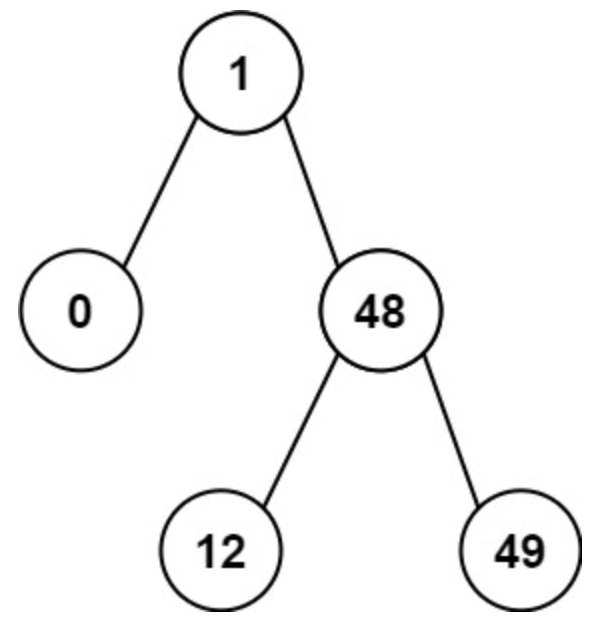
\includegraphics[width=0.25\linewidth]{images/lc0530_example}
	\label{fig:lc0530example}
\end{figure}
{\colorbox{CodeBackground}{\lstinline|--> 1|}}

\subsection*{Solution 1 - In-order Traversal (Recursive)}
\begin{lstlisting}
int getMinimumDifference(TreeNode* root) {
	int min_diff = std::numeric_limits<int>::max();
	TreeNode* prev = nullptr;
	InorderTraverse(root, prev, min_diff);
	return min_diff;
}

void InorderTraverse(TreeNode* node, TreeNode*& prev, int& min_diff) {
	if (!node) { return; }
	InorderTraverse(node->left, prev, min_diff);
	if (prev) { min_diff = std::min(min_diff, node->val - prev->val); }
	prev = node;
	InorderTraverse(node->right, prev, min_diff);
}
\end{lstlisting}

\subsection*{Solution 2 - In-order Traversal (Iterative)}
\begin{lstlisting}
int getMinimumDifference(TreeNode* root) {
	if (!root) { return -1; }
	std::stack<TreeNode*> stk;
	TreeNode* curr = root;
	TreeNode* prev = nullptr;
	int min_diff = std::numeric_limits<int>::max();
	while (curr || !stk.empty()) {
		while (curr) {
			stk.push(curr);
			curr = curr->left;
		}
		TreeNode* top = stk.top();
		stk.pop();
		if (prev) { min_diff = std::min(min_diff, top->val - prev->val); }
		prev = top;
		curr = top->right;
	}
	return min_diff;
}
\end{lstlisting}

\section{LC 0173 - BST Iterator}
Implement the {\colorbox{CodeBackground}{\lstinline|BSTIterator|}} class that represents an iterator over the \ul{in-order traversal} of a \ul{binary search tree (BST)}:
\begin{itemize}
	\item {\colorbox{CodeBackground}{\lstinline|BSTIterator(TreeNode root)|}} - Initializes an object of the {\colorbox{CodeBackground}{\lstinline|BSTIterator|}} class. The {\colorbox{CodeBackground}{\lstinline|root|}} of the BST is given as part of the constructor. The pointer should be initialized to a non-existent number smaller than any element in the BST.
	\item {\colorbox{CodeBackground}{\lstinline|int next()|}} - Moves the pointer to the right, then returns the number at the pointer. Notice that the first call to {\colorbox{CodeBackground}{\lstinline|next()|}} will return the smallest element in the BST.
	\item {\colorbox{CodeBackground}{\lstinline|boolean hasNext()|}} - Returns {\colorbox{CodeBackground}{\lstinline|true|}} if there exists a number in the traversal to the right of the pointer, otherwise returns {\colorbox{CodeBackground}{\lstinline|false|}}.
\end{itemize}


\begin{lstlisting}
class BSTIterator {
 public:
	BSTIterator(TreeNode* root) { PushAll(root); }
	
	/** @return the next smallest number */
	int next() {
		TreeNode* top = stk.top();
		stk.pop();
		PushAll(top->right);
		return top->val;
	}
	
	/** @return whether we have a next smallest number */
	bool hasNext() { return !stk.empty(); }
	
 private:
	void PushAll(TreeNode* node) {
		while (node) {
			stk.push(node);
			node = node->left;
		}
	}
	
	std::stk<TreeNode*> stk;
};
\end{lstlisting}

\section{LC 0235 - Lowest Common Ancestor of a BST}\label{lc0235}
Given a \ul{binary search tree (BST)}, find the \ul{lowest common ancestor (LCA)} node of two given nodes in the BST. Note that both {\colorbox{CodeBackground}{\lstinline|p|}} and {\colorbox{CodeBackground}{\lstinline|q|}} are in the tree and {\colorbox{CodeBackground}{\lstinline|p != q|}}.\\

Definition of LCA: The \ul{lowest common ancestor (LCA)} is defined between two nodes {\colorbox{CodeBackground}{\lstinline|p|}} and {\colorbox{CodeBackground}{\lstinline|q|}} as the lowest node in the tree that has both {\colorbox{CodeBackground}{\lstinline|p|}} and {\colorbox{CodeBackground}{\lstinline|q|}} as \ul{descendants} (where we allow a node to be a \ul{descendant} of itself). \\

Example:

\begin{figure}[H]
	\centering
	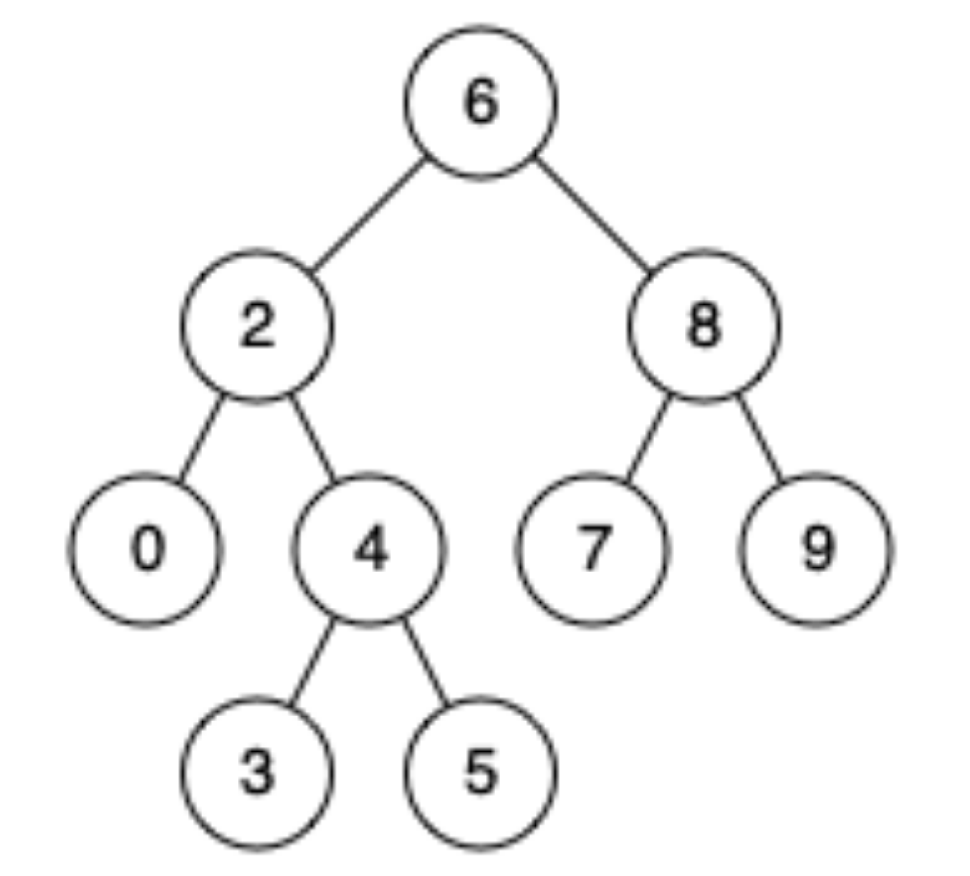
\includegraphics[width=0.3\linewidth]{images/lc0235_example}
	\label{fig:lc0235example}
\end{figure}
\begin{lstlisting}
	p = 2, q = 8 --> 6
	p = 2, q = 4 --> 2
\end{lstlisting}

\subsection*{Solution}
\begin{lstlisting}
TreeNode* lowestCommonAncestor(TreeNode* root, TreeNode* p, TreeNode* q) {
	TreeNode* curr = root;
	while (curr) {
		if (p->val > curr->val && q->val > curr->val) {
			curr = curr->right;
		} else if (p->val < curr->val && q->val < curr->val) {
			curr = curr->left;
		} else {
			return curr;
		}
	}
	return nullptr;
}
\end{lstlisting}

\subsection*{Related}
\begin{itemize}
	\item \hyperref[lc0236]{LC 0236 - Lowest Common Ancestor of a Binary Tree}
	\item \hyperref[lc0235]{LC 0235 - Lowest Common Ancestor of a BST}
\end{itemize}

\section{LC 0110 - Balanced Binary Tree}
Given a \ul{binary tree}, determine if it is \ul{height-balanced}.

\section{LC 0257 - Binary Tree Paths}
Given the {\colorbox{CodeBackground}{\lstinline|root|}} of a \ul{binary tree}, return all \ul{root-to-leaf paths} in any order.\\

\begin{itemize}
\item Example 1: {\colorbox{CodeBackground}{\lstinline|root = [1,2,3,null,5] --> ["125","13"]|}}
\begin{figure}[H]
\centering
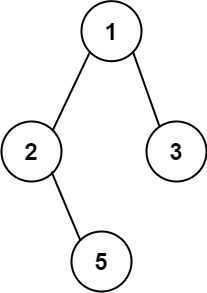
\includegraphics[width=0.16\linewidth]{images/lc0257_eg}
\label{fig:lc0257eg}
\end{figure}
\item Example 2: {\colorbox{CodeBackground}{\lstinline|root = [1] --> ["1"]|}}
\end{itemize}

\section{LC 0404 - Sum of Left Leaves}
Given the {\colorbox{CodeBackground}{\lstinline|root|}} of a \ul{binary tree}, return the sum of all left leaves.\\

\begin{itemize}
\item Example 1: {\colorbox{CodeBackground}{\lstinline|root = [3,9,20,null,null,15,7] --> 24 (9 + 15)|}}
\begin{figure}[H]
\centering
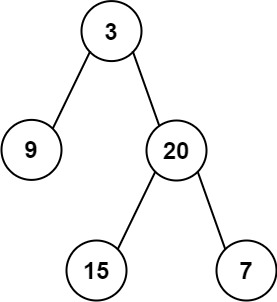
\includegraphics[width=0.22\linewidth]{images/lc0404_eg}
\label{fig:lc0404eg}
\end{figure}
\item Example 2: {\colorbox{CodeBackground}{\lstinline|root = [1] --> 0|}}
\end{itemize}

\section{LC 0513 - Find Bottom Left Tree Value}
Given the {\colorbox{CodeBackground}{\lstinline|root|}} of a\ul{ binary tree}, return the leftmost value \ul{in the last row of the tree}.

\begin{itemize}
\item Example 1: {\colorbox{CodeBackground}{\lstinline|root = [2,1,3] --> 1|}}
\begin{figure}[H]
\centering
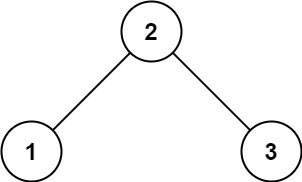
\includegraphics[width=0.25\linewidth]{images/lc0513_eg1}
\label{fig:lc0513eg1}
\end{figure}
\item Example 2: {\colorbox{CodeBackground}{\lstinline|root = [1,2,3,4,null,5,6,null,null,7] --> 7|}}
\begin{figure}[H]
\centering
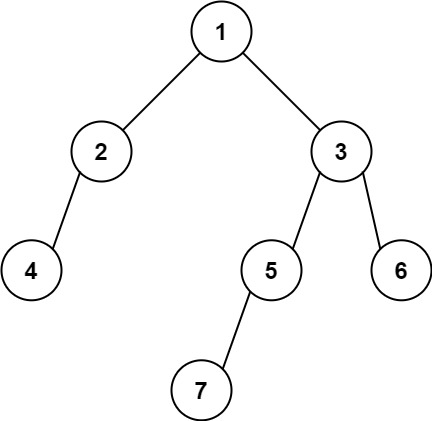
\includegraphics[width=0.35\linewidth]{images/lc0513_eg2}
\label{fig:lc0513eg2}
\end{figure}
\end{itemize}

\section{LC 0654 - Maximum Binary Tree}
You are given an integer array {\colorbox{CodeBackground}{\lstinline|nums|}} with no duplicates. A maximum binary tree can be built recursively from {\colorbox{CodeBackground}{\lstinline|nums|}} using the following algorithm:
\begin{itemize}
\item Create a root node whose value is the maximum value in {\colorbox{CodeBackground}{\lstinline|nums|}}.
\item Recursively build the left subtree on the subarray prefix to the left of the maximum value.
\item Recursively build the right subtree on the subarray suffix to the right of the maximum value.
\end{itemize}
Return the maximum binary tree built from {\colorbox{CodeBackground}{\lstinline|nums|}}.\\

\begin{itemize}
\item Example 1: {\colorbox{CodeBackground}{\lstinline|nums = [3,2,1,6,0,5]|}}
\begin{figure}[H]
\centering
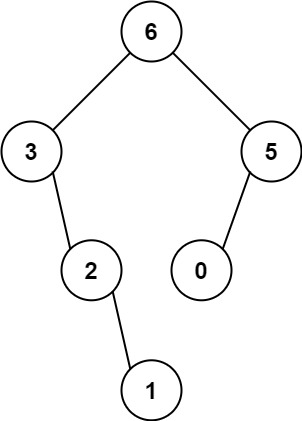
\includegraphics[width=0.25\linewidth]{images/lc0654_eg1}
\label{fig:lc0654eg1}
\end{figure}
\item Example 2: {\colorbox{CodeBackground}{\lstinline|nums = [3,2,1]|}}
\begin{figure}[H]
\centering
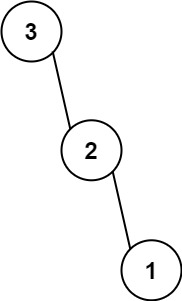
\includegraphics[width=0.15\linewidth]{images/lc0654_eg2}
\label{fig:lc0654eg2}
\end{figure}
\end{itemize}

\section{LC 0617 - Merge Two Binary Trees}

\section{LC 0700 - Search in a Binary Search Tree}

\section{LC 0501 - Find Mode in Binary Search Tree}

\section{LC 0701 - Insert into a Binary Search Tree}

\section{LC 0450 - Delete Node in a BST}

\section{LC 0669 - Trim a Binary Search Tree}

\section{LC 0108 - Convert Sorted Array to Binary Search Tree}

\section{LC 0538 - Convert BST to Greater Tree}

\section{LC 0107 - Binary Tree Level Order Traversal II}

\section{LC 0429 - N-ary Tree Level Order Traversal}

\section{LC 0515 - Find Largest Value in Each Tree Row}

\section{LC 0116 - Populating Next Right Pointers in Each Node}